\documentclass{article}

% Official NeurIPS 2026 workshop modes require [sglblindworkshop] or
% [dblblindworkshop] together with a real \workshoptitle{...}. No official
% 2026 workshop CFP or accepted-workshop title matching this paper was public
% on April 8, 2026, so this artifact stays in generic preprint mode.
\usepackage[preprint]{neurips_2026}
\usepackage[utf8]{inputenc}
\usepackage[T1]{fontenc}
\usepackage{hyperref}
\usepackage{url}
\usepackage{booktabs}
\usepackage{amsfonts}
\usepackage{nicefrac}
\usepackage{microtype}
\usepackage{xcolor}
\usepackage{graphicx}
\usepackage{amsmath,amssymb,mathtools}
\usepackage{enumitem}

\title{When Does Policy-Level Permutation Consistency Help Zero-Shot Coordination?\\A Controlled Study in Small MARL}

\author{%
  Raj Kashikar \\
  Virginia Tech \\
  \texttt{rajskashikar@vt.edu}
}

\newcommand{\method}{PICR-MA}
\newcommand{\KL}{\mathrm{KL}}
\newcommand{\JS}{\mathrm{JS}}
\newcommand{\E}{\mathbb{E}}

\begin{document}

\maketitle

\begin{abstract}
Arbitrary teammate ordering is a hidden nuisance variable in decentralized MARL: a vanilla MLP can treat the ``first'' teammate differently from the ``second'' even when teammates are exchangeable. We study whether reducing that dependence improves held-out partner coordination. Our method, \emph{PICR-MA}, is a lightweight actor-side regularizer that samples two independent permutations of teammate feature blocks and penalizes the symmetric Kullback--Leibler divergence between the resulting action distributions, leaving the inference-time policy unchanged. We evaluate \method\ against IPPO, Deep Sets, and Other-Play on a 5-seed, 50k-step PettingZoo MPE cohort (\texttt{simple\_spread\_v3}, \texttt{simple\_adversary\_v3}), with pilot ablations and checkpoint-based cross-play against 19 held-out partners per ego policy. \method\ reliably lowers permutation sensitivity, but the coordination effect is environment-dependent: relative to IPPO, same-family held-out cross-play rises on \texttt{simple\_adversary\_v3} (+2.73 mean paired delta, wide 95\% bootstrap CI) and falls on \texttt{simple\_spread\_v3} (-1.56, CI excludes zero). Paired-seed analyses therefore reveal a consistent diagnostic shift but not a consistent coordination improvement. The workshop contribution is a controlled empirical result: policy-level permutation consistency is a useful bias to measure and sometimes exploit, yet lower teammate-order sensitivity is not a reliable standalone proxy for zero-shot coordination quality.
\end{abstract}

\section{Introduction}
Zero-shot coordination (ZSC) asks whether an agent trained in self-play can cooperate with an unfamiliar partner at test time \citep{hu2020otherplay}. In decentralized MARL, one source of ZSC brittleness is mundane but pervasive: teammate features are commonly fed to a multilayer perceptron in a fixed concatenation order, so the policy may learn distinct roles for the ``first'' and ``second'' teammate even when the environment is symmetric. This creates an avoidable dependence on an arbitrary observation convention.

This paper studies a minimal intervention at the policy level. Rather than changing the policy architecture to a set encoder or graph network \citep{zaheer2017deepsets, liu2020pic}, we regularize the policy to produce similar action distributions under different teammate-order views of the same observation. The resulting method, \method, is intentionally simple: during training we apply two independent permutations to teammate feature blocks and penalize their action-distribution disagreement with a symmetric KL loss. The design goal is not exact invariance by construction; it is to inject a soft symmetry bias into an otherwise ordinary shared-parameter MLP.

The central question is not only whether this penalty reduces a permutation-sensitivity diagnostic. The more important question is whether that diagnostic reduction improves downstream coordination with held-out partners. The answer in our controlled study is informative but non-universal. On \texttt{simple\_adversary\_v3}, \method\ raises the cohort-average same-family held-out cross-play score over IPPO while also lowering permutation sensitivity, but the matched-seed gains are unstable. On \texttt{simple\_spread\_v3}, it lowers permutation sensitivity in every paired comparison and still loses on held-out coordination in every pair. This separation between ``more order-consistent'' and ``better coordinated'' is the main scientific point of the paper.

\paragraph{Contributions.}
\begin{itemize}[leftmargin=1.3em]
\item We implement \method\ as a policy-side permutation-consistency regularizer for shared-parameter decentralized MARL with no inference-time architectural change.
\item We evaluate it with a controlled held-out partner protocol that separates same-family and cross-family cross-play, uses explicit teammate-block slicing, and reports paired-seed uncertainty rather than only leaderboard averages.
\item We show that \method\ reliably reduces permutation sensitivity in the main MPE cohort, but its effect on held-out coordination is environment-dependent: helpful on \texttt{simple\_adversary\_v3} and harmful on \texttt{simple\_spread\_v3}.
\item We identify a concrete diagnostic failure mode for symmetry-aware MARL: lower teammate-order sensitivity is informative, but it is not a reliable standalone proxy for zero-shot coordination quality.
\end{itemize}

\section{Related Work and Positioning}
\paragraph{Zero-shot coordination and partner generalization.}
ZSC asks whether independently trained agents can coordinate without test-time communication or adaptation. Other-Play addresses this problem by randomizing over symmetry-equivalent conventions during training \citep{hu2020otherplay}. Our evaluation protocol adopts the same held-out partner mindset, but the mechanism is different: \method\ regularizes policy outputs under teammate permutations rather than randomizing role assignments or conventions at the trajectory level.

\paragraph{Symmetry-aware MARL architectures.}
A common response to exchangeable inputs is to change the network architecture. Deep Sets provide exact permutation invariance at the encoder level \citep{zaheer2017deepsets}, and prior MARL work has applied permutation-invariant critics to reduce agent-order sensitivity under centralized training \citep{liu2020pic}. By contrast, many practical MARL baselines still process ordered agent features with conventional actors or critics \citep{lowe2017maddpg, sunehag2018vdn, rashid2018qmix, terry2020ps}. \method\ targets this regime: the actor stays an ordinary shared-parameter MLP at inference time, and the symmetry bias enters only through the training loss.

\paragraph{Consistency regularization.}
The regularizer is also related in spirit to consistency penalties in semi-supervised learning, where multiple views of the same example are encouraged to produce similar predictions \citep{tarvainen2017meanteacher, sohn2020fixmatch}. The difference here is structural rather than cosmetic: the two views are teammate-order permutations of a MARL observation, and the scientific question is not only whether the policy becomes more self-consistent, but whether that self-consistency transfers to better held-out partner coordination. That diagnostic-versus-outcome gap is the main empirical claim of the paper.

\begin{figure*}[t]
\centering
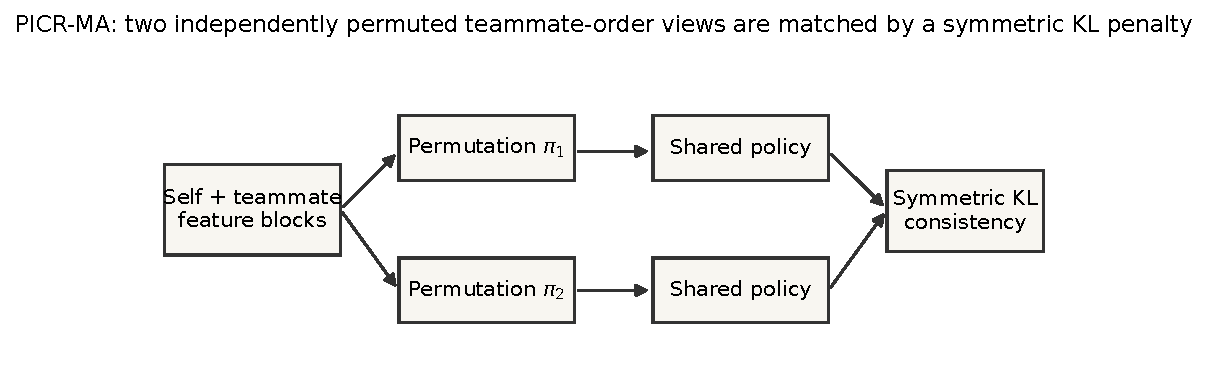
\includegraphics[width=0.92\linewidth]{latex/figures/method_overview.pdf}
\caption{\method\ overview. For each training example, the teammate-specific observation blocks are permuted twice, the shared policy is evaluated on both views, and the resulting action distributions are matched with a symmetric KL penalty. Inference uses the original policy with no extra architectural machinery.}
\label{fig:method}
\end{figure*}

\section{Method}
Each agent observation is decomposed into non-teammate features $s$ and teammate-specific blocks $U = [u_1,\dots,u_{n-1}]$. For two independently sampled teammate permutations $\pi_1$ and $\pi_2$, we form
\begin{align}
o_{(1)} &= [s \Vert \pi_1(U)], &
p_1 &= \pi_\theta(\cdot \mid o_{(1)}), \\
o_{(2)} &= [s \Vert \pi_2(U)], &
p_2 &= \pi_\theta(\cdot \mid o_{(2)}).
\end{align}
The regularizer is
\begin{align}
\mathcal{L}_{\text{\method}} =
\lambda \, \E \Big[
\tfrac{1}{2}\KL(p_1 \Vert p_2) +
\tfrac{1}{2}\KL(p_2 \Vert p_1)
\Big].
\end{align}
The training objective is $\mathcal{L}_{\text{RL}} + \mathcal{L}_{\text{\method}}$, where $\mathcal{L}_{\text{RL}}$ is the base on-policy objective. We use a soft symmetric-KL penalty rather than exact set pooling because the goal is to bias the actor toward exchangeability without rewriting the deployed architecture. The implementation keeps the base MLP policy unchanged at inference time; the only overhead is the additional training-time forward passes required for the consistency term. The penalty is applied only to teammate blocks designated as exchangeable by the environment-specific slicing metadata; self features and task-asymmetric features are left untouched.

We also implement teammate dropout as an ablation that zeros a random subset of teammate blocks during training. It is not part of the core method and, empirically, it does not strengthen the story.

\section{Experimental Setup and Statistics}
\paragraph{Environments.}
The main evidence comes from two PettingZoo MPE tasks \citep{terry2021pettingzoo}: \texttt{simple\_spread\_v3}, a fully cooperative three-agent coverage task, and \texttt{simple\_adversary\_v3}, where a cooperative team interacts with an adversary. In \texttt{simple\_spread\_v3}, all cooperative agents are treated as exchangeable. In \texttt{simple\_adversary\_v3}, only the good-agent team is treated as exchangeable; the adversary is evaluated with its own policy and is not regularized. Matrix coordination and stag-hunt variants are retained as fast sanity checks and are reported in the appendix rather than driving the main claim.

\paragraph{Baselines.}
We compare four methods under matched training budgets: IPPO, IPPO+\method, IPPO with a Deep Sets encoder, and Other-Play-style teammate-order randomization \citep{schulman2017ppo, terry2020ps, zaheer2017deepsets, hu2020otherplay}. The comparison is intentionally practical: Deep Sets provides an architectural invariance baseline, and Other-Play provides a symmetry-randomization baseline with a stronger ZSC pedigree.

\paragraph{Main cohort and pilot ablations.}
The main MPE cohort uses 5 seeds, 50k environment steps per seed, and held-out partner evaluation from independently trained policies sharing the same run tag. A 20k, 3-seed pilot sweep selected $\lambda \in \{0.02, 0.05, 0.10\}$ for \method\ and evaluated teammate dropout at probability $0.1$. The main 50k PICR-MA setting uses $\lambda=0.02$ because it gave the strongest held-out cross-play among the pilot settings, even though larger $\lambda$ values reduced $\JS$ more aggressively.

\paragraph{Evaluation.}
For each run we record training return, held-out partner cross-play return, permutation sensitivity measured by Jensen--Shannon divergence under teammate-order swaps, and environment-specific diagnostics such as collisions or goal-margin statistics. Each main-cohort ego policy is evaluated against every compatible checkpoint from the same environment and run tag except itself, yielding 19 held-out partners per ego policy: 4 same-family and 15 cross-family. Every ego--partner pair is run for 16 greedy episodes from fresh seeds. The headline cross-play number in the main table is same-family held-out cross-play, because it directly asks whether a training-time inductive bias stabilizes coordination with independently trained partners that share the same method family. Cross-family partners are reported separately in the appendix. Cross-play results are produced from saved checkpoints with a partner-pool filter that excludes the evaluated run itself and respects the intended run tag.

\paragraph{Statistical treatment.}
Tables report mean $\pm$ standard error across seeds unless noted otherwise. For the key IPPO$\rightarrow$\method\ comparison we also report matched-seed deltas with 10{,}000-sample nonparametric bootstrap confidence intervals, because the scientific question is directional consistency rather than leaderboard ranking alone.

\paragraph{Implementation and compute.}
All experiments were executed sequentially on a single Apple Silicon laptop under the repo's lean-safe resource profile. The learner is a compact NumPy actor--critic implementation, which keeps the artifact easy to inspect and reproduce on commodity hardware. IPPO, \method, and Other-Play share the same MLP backbone and optimization budget, so \method's extra cost comes from two additional training-time forward passes rather than a larger inference model; only Deep Sets changes capacity (1606 versus 3302 cooperative parameters on \texttt{simple\_spread\_v3}, and 1350 versus 3238 on \texttt{simple\_adversary\_v3}). We revisit the scale consequences of this implementation choice in the limitations discussion rather than treating them as hidden caveats.

\section{Results}
\paragraph{Permutation consistency is real.}
Table~\ref{tab:main-results} and Figure~\ref{fig:perm} show that \method\ does what it is supposed to do mechanically. In the main 50k cohort, it lowers teammate-order sensitivity relative to IPPO on both MPE tasks, from $0.0263 \pm 0.0063$ to $0.0127 \pm 0.0019$ on \texttt{simple\_spread\_v3} and from $0.0102 \pm 0.0066$ to $0.0053 \pm 0.0025$ on \texttt{simple\_adversary\_v3}. Deep Sets drives this diagnostic to zero, as expected for an architectural invariance baseline.

\begin{table*}[t]
\centering
\caption{Main 50k-step, 5-seed MPE results (mean $\pm$ standard error). The cross-play column reports same-family held-out partner cross-play over 4 held-out same-family partners per ego policy; lower JS is better. For \texttt{simple\_spread\_v3}, the task diagnostic is collision rate (lower is better); for \texttt{simple\_adversary\_v3}, it is cooperative goal margin (higher is better). Best same-family cross-play and best JS within each environment are bolded.}
\label{tab:main-results}
\resizebox{\textwidth}{!}{\begin{tabular}{llcccc}
\toprule
Environment & Method & Train return & Same-family cross-play & JS $\downarrow$ & Env metric \\
\midrule
Simple Adversary & IPPO & 2.346 $\pm$ 1.813 & 17.429 $\pm$ 3.770 & 0.010 $\pm$ 0.007 & margin=0.260 \\
Simple Adversary & PICR-MA & 6.585 $\pm$ 3.502 & 20.159 $\pm$ 2.043 & 0.005 $\pm$ 0.003 & margin=0.345 \\
Simple Adversary & Deep Sets & 7.965 $\pm$ 1.698 & 11.356 $\pm$ 3.244 & 0.000 $\pm$ 0.000 & margin=0.392 \\
Simple Adversary & Other-Play & 3.603 $\pm$ 1.497 & 20.934 $\pm$ 3.429 & 0.014 $\pm$ 0.007 & margin=0.310 \\
\midrule
Simple Spread & IPPO & -21.952 $\pm$ 0.472 & -25.649 $\pm$ 0.271 & 0.026 $\pm$ 0.006 & coll=0.164 \\
Simple Spread & PICR-MA & -23.425 $\pm$ 0.625 & -27.206 $\pm$ 0.730 & 0.013 $\pm$ 0.002 & coll=0.155 \\
Simple Spread & Deep Sets & -24.776 $\pm$ 1.413 & -25.550 $\pm$ 0.489 & 0.000 $\pm$ 0.000 & coll=0.065 \\
Simple Spread & Other-Play & -21.626 $\pm$ 0.209 & -25.533 $\pm$ 0.566 & 0.025 $\pm$ 0.013 & coll=0.079 \\
\bottomrule
\end{tabular}
}
\end{table*}

\begin{figure*}[t]
\centering
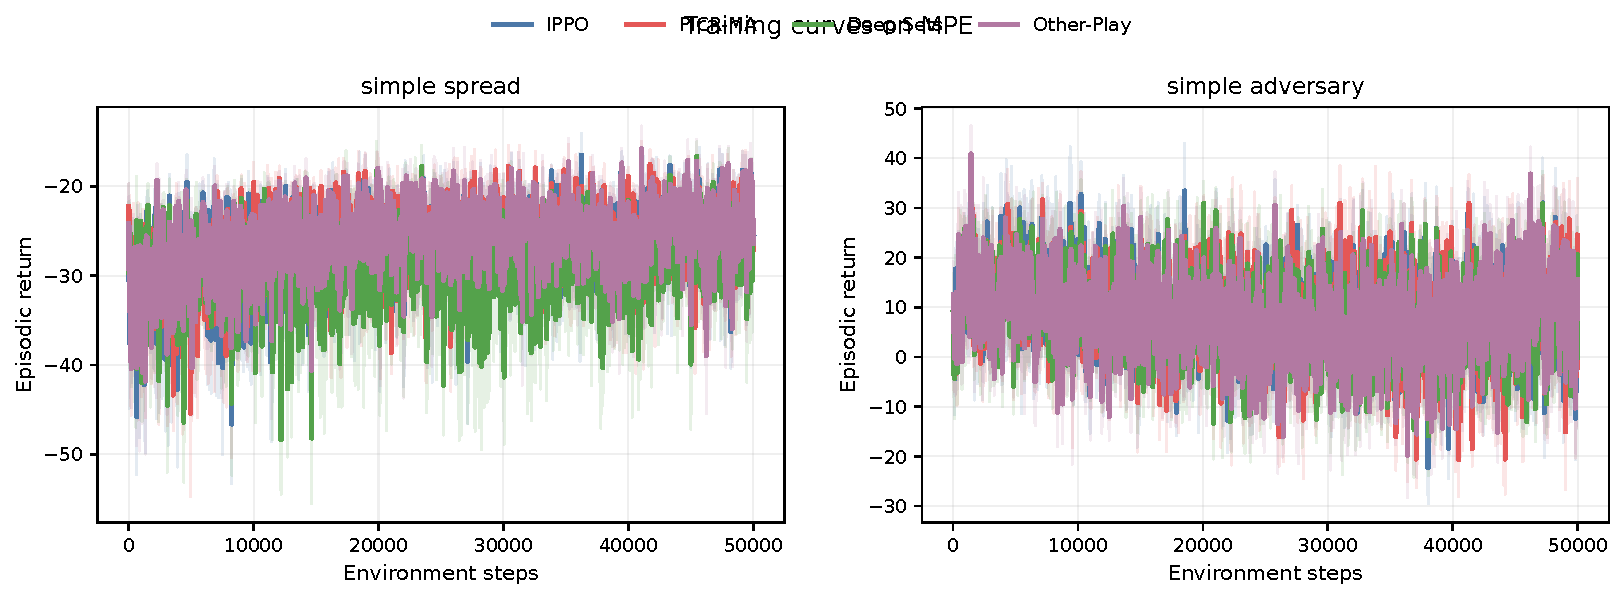
\includegraphics[width=0.95\linewidth]{latex/figures/learning_curves_mpe.pdf}
\caption{MPE learning curves for the main 50k cohort. Solid lines show means across 5 seeds and shaded regions show standard error. The curves also make a substantive point for interpretation: \texttt{simple\_spread\_v3} is still improving late in training, so a mild symmetry bias can interact with partially learned coordination conventions rather than only with converged policies.}
\label{fig:curves}
\end{figure*}

\paragraph{Permutation consistency is reliable; coordination gains are not.}
The main table quantifies the split outcome directly. On \texttt{simple\_adversary\_v3}, same-family held-out cross-play rises from $17.429 \pm 3.770$ for IPPO to $20.159 \pm 2.043$ for \method\ while permutation sensitivity drops from $0.0102 \pm 0.0066$ to $0.0053 \pm 0.0025$. On \texttt{simple\_spread\_v3}, \method\ again cuts permutation sensitivity, from $0.0263 \pm 0.0063$ to $0.0127 \pm 0.0019$, yet same-family held-out cross-play falls from $-25.649 \pm 0.271$ to $-27.206 \pm 0.730$. The regularizer therefore behaves consistently as a diagnostic intervention, but not as a universal coordination improvement.

\paragraph{Lower sensitivity does not reliably imply better coordination.}
Figure~\ref{fig:zsc-mismatch} sharpens this point with matched IPPO$\rightarrow$\method\ seed pairs. On \texttt{simple\_spread\_v3}, \method\ lowers $\JS$ in all five paired comparisons but loses on same-family held-out cross-play in all five; the mean cross-play delta is $-1.557$ with a 95\% bootstrap interval of $[-3.013, -0.651]$. On \texttt{simple\_adversary\_v3}, \method\ lowers $\JS$ in four of five pairs and improves same-family held-out cross-play in three of five; the mean cross-play delta is $+2.731$ with a wide 95\% bootstrap interval of $[-6.141, 12.263]$. The positive adversary result is therefore real at the cohort-average level but much less stable than the diagnostic change, which is exactly the mismatch this paper wants to make concrete.

\begin{figure*}[t]
\centering
\begin{minipage}[t]{0.48\linewidth}
\centering
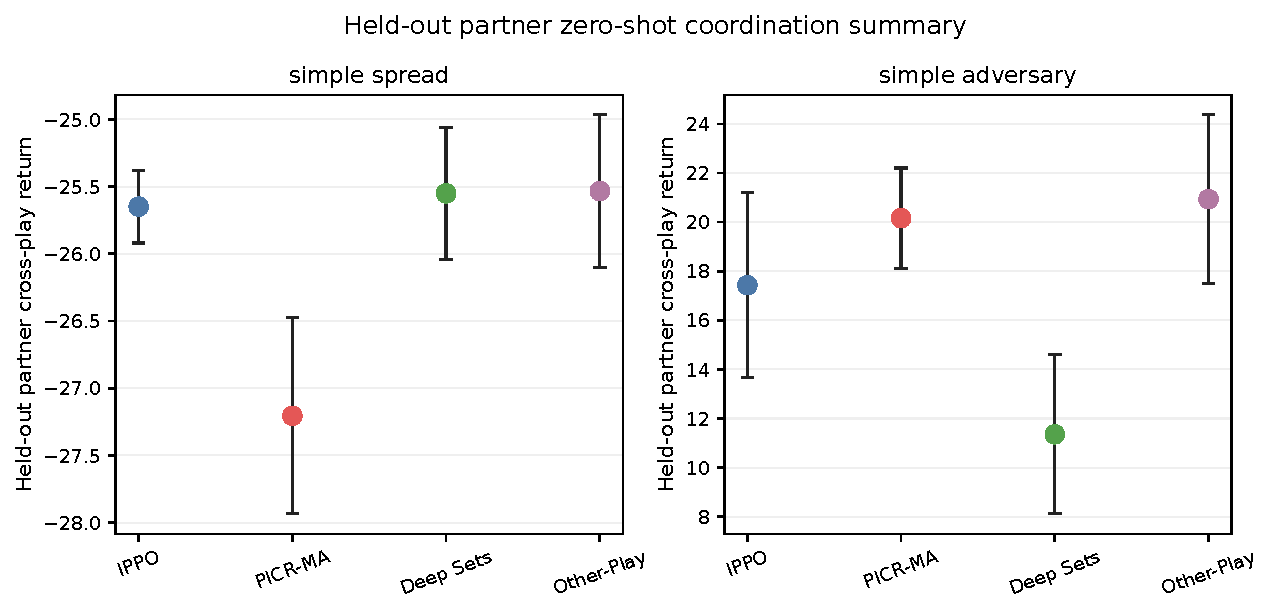
\includegraphics[width=\linewidth]{latex/figures/zero_shot_crossplay_summary.pdf}
\end{minipage}\hfill
\begin{minipage}[t]{0.48\linewidth}
\centering
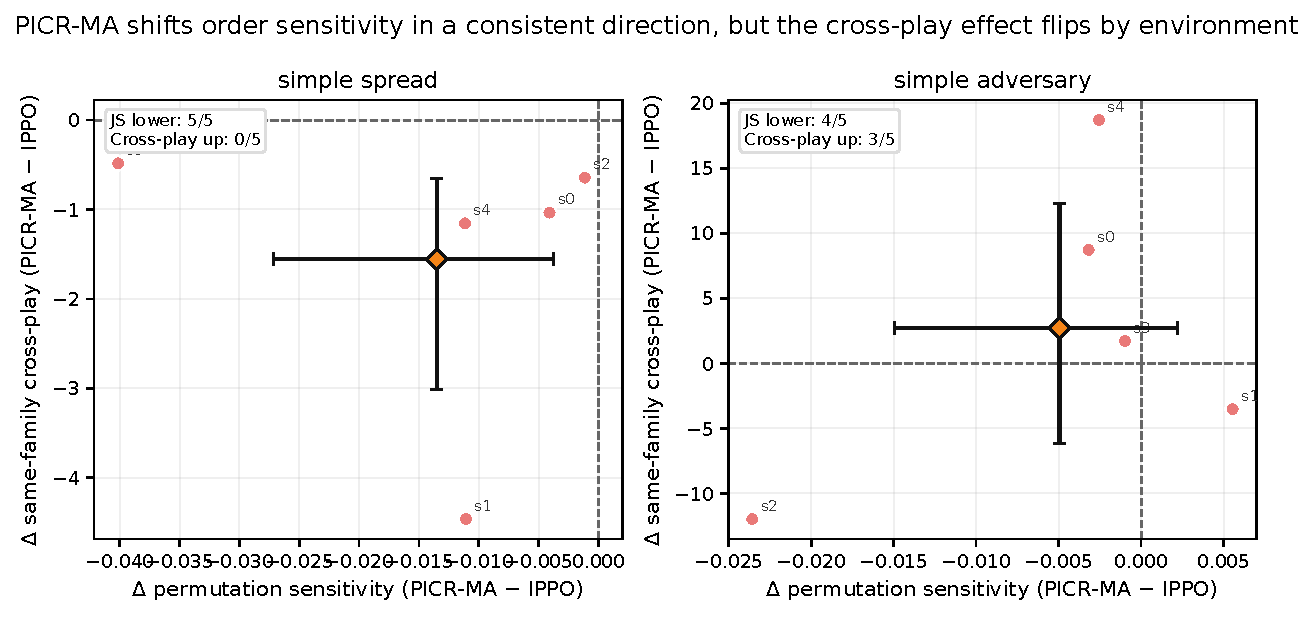
\includegraphics[width=\linewidth]{latex/figures/invariance_coordination_mismatch.pdf}
\end{minipage}
\caption{Left: same-family held-out partner ZSC summary for the main cohort. Right: matched IPPO$\rightarrow$\method\ seed-pair deltas; the diamond marks the mean paired delta and the error bars show a 95\% bootstrap interval over seeds. \method\ moves permutation sensitivity leftward on both tasks, but the associated cross-play shift is positive only inconsistently on \texttt{simple\_adversary\_v3} and negative in every \texttt{simple\_spread\_v3} pair.}
\label{fig:zsc-mismatch}
\end{figure*}

\begin{figure}[t]
\centering
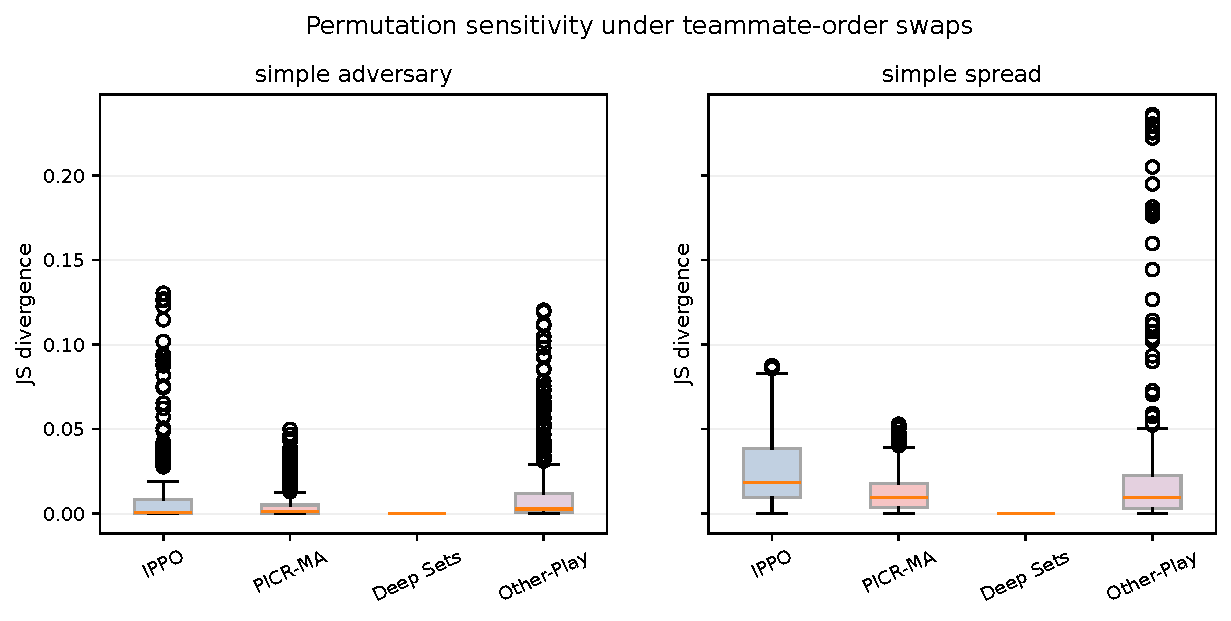
\includegraphics[width=\linewidth]{latex/figures/permutation_sensitivity_results.pdf}
\caption{Permutation sensitivity distributions over saved evaluation states. Deep Sets is exactly invariant by construction; \method\ substantially improves over IPPO on both MPE tasks, making the subsequent coordination mismatch harder to dismiss as a measurement artifact.}
\label{fig:perm}
\end{figure}

\paragraph{Baselines matter.}
The baseline story is instructive rather than uniform. Deep Sets is the strongest invariance baseline but is weak on \texttt{simple\_adversary\_v3} held-out cross-play, suggesting that exact invariance alone can remove useful asymmetries in that environment. Other-Play is slightly stronger than \method\ on \texttt{simple\_adversary\_v3} and clearly stronger on \texttt{simple\_spread\_v3}. The appendix cross-family breakdown further shows that \method's positive adversary signal is concentrated in same-family partners rather than a uniform gain across partner families. The practical takeaway is therefore narrower than a leaderboard claim: \method\ occupies a simplicity--performance niche in which a soft policy-side bias can be competitive without demanding an architectural rewrite.

\paragraph{Ablations favor mild regularization.}
The 20k pilot ablations in Table~\ref{tab:ablation} show that stronger regularization does not monotonically help. On \texttt{simple\_spread\_v3}, increasing $\lambda$ reduces $\JS$ but steadily worsens held-out cross-play. On \texttt{simple\_adversary\_v3}, the mild setting $\lambda=0.02$ gives the best held-out cross-play in the sweep. Teammate dropout harms both tasks. Runtime overhead is moderate rather than negligible: in the main 50k cohort, \method\ costs $1.62\times$ IPPO on \texttt{simple\_spread\_v3} and $1.33\times$ IPPO on \texttt{simple\_adversary\_v3}, while remaining well below the Deep Sets cost on \texttt{simple\_spread\_v3}.

\begin{table}[t]
\centering
\caption{PICR-MA pilot ablations from the 20k, 3-seed sweep (mean $\pm$ standard error). The cross-play column reports same-family held-out partner cross-play. Bold entries mark the best cross-play and best JS within each environment. The table supports a narrow but useful claim: mild regularization is preferable, and teammate dropout is not helpful in this study.}
\label{tab:ablation}
\resizebox{\linewidth}{!}{\begin{tabular}{llccc}
\toprule
Environment & Setting & Same-family cross-play & JS $\downarrow$ & Runtime (s) \\
\midrule
Simple Spread & $\lambda=0.02$ & -31.673 $\pm$ 0.520 & 0.025 $\pm$ 0.006 & 35.936 \\
Simple Spread & $\lambda=0.05$ & -33.884 $\pm$ 1.281 & 0.022 $\pm$ 0.004 & 55.688 \\
Simple Spread & $\lambda=0.10$ & -34.673 $\pm$ 1.060 & 0.009 $\pm$ 0.002 & 91.293 \\
Simple Spread & dropout $p=0.10$ & -37.486 $\pm$ 2.504 & 0.016 $\pm$ 0.004 & 14.812 \\
\midrule
Simple Adversary & $\lambda=0.02$ & 25.743 $\pm$ 1.344 & 0.016 $\pm$ 0.006 & 50.579 \\
Simple Adversary & $\lambda=0.05$ & 22.688 $\pm$ 3.005 & 0.012 $\pm$ 0.002 & 66.191 \\
Simple Adversary & $\lambda=0.10$ & 24.743 $\pm$ 2.973 & 0.011 $\pm$ 0.003 & 39.520 \\
Simple Adversary & dropout $p=0.10$ & 16.897 $\pm$ 2.086 & 0.026 $\pm$ 0.016 & 18.596 \\
\bottomrule
\end{tabular}
}
\end{table}

\begin{figure}[t]
\centering
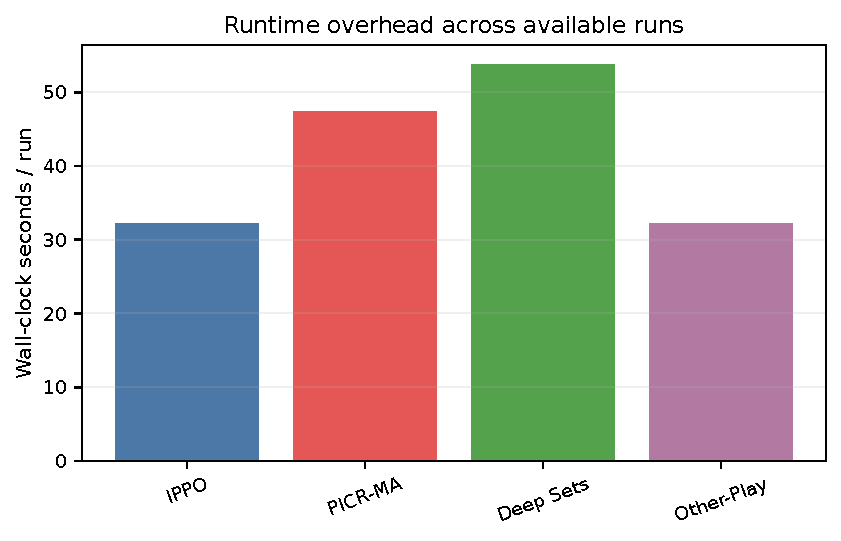
\includegraphics[width=\linewidth]{latex/figures/runtime_overhead.pdf}
\caption{Per-run wall-clock runtime across the main cohort. PICR-MA is meaningfully more expensive than IPPO, but it pays for extra training-time consistency passes rather than a larger deployed actor and remains cheaper than Deep Sets on \texttt{simple\_spread\_v3}.}
\label{fig:runtime}
\end{figure}

\section{Discussion, Limitations, and Broader Impact}
This paper should not be read as evidence that policy-level permutation consistency is a new default recipe for ZSC in MARL. The stronger and more interesting conclusion is narrower: it is possible to reduce order sensitivity substantially with a very small policy-side intervention, but the downstream value of that intervention depends strongly on the environment and the competing inductive biases already present in the baseline. For workshop purposes, that is still a useful result. It turns a vague intuition about symmetry into a controlled measurement problem and shows that the resulting diagnostic can move more reliably than the coordination outcome that practitioners actually care about.

The contrast between the two MPE tasks suggests a practical hypothesis. In \texttt{simple\_adversary\_v3}, reducing brittle teammate-order dependence appears helpful because the cooperative team benefits from a mild symmetry bias without requiring exact exchangeability. In \texttt{simple\_spread\_v3}, the same bias does not rescue coordination and may suppress distinctions that matter for coverage conventions such as emergent spatial role assignment. The paired-delta analysis makes this concrete: the same intervention moves the diagnostic in the intended direction on both tasks, yet the coordination effect flips sign by environment and does not generalize cleanly across partner families. Invariance diagnostics measure one property of the policy, but they do not summarize the entire coordination problem.

\paragraph{Limitations.}
The learner is a compact NumPy implementation rather than a standard PyTorch PPO codebase. The main MPE cohort is stronger than the original smoke runs, but it remains a 50k-step laptop-scale study rather than a large benchmark campaign. The paper also centers same-family held-out coordination as its primary endpoint; that choice is scientifically motivated, but it means the strongest positive signal is not a universal cross-family gain. Matrix games are useful sanity checks, not headline evidence. These limitations support a focused workshop claim rather than a broader declaration that permutation consistency is the right default inductive bias for MARL.

\paragraph{Broader impact.}
On the positive side, the paper argues for more careful robustness diagnostics in multi-agent learning and makes a reproducible case that a seemingly attractive metric can fail as a proxy for coordination quality. On the negative side, any method that improves the reliability of decentralized coordination could eventually benefit deployed multi-agent systems in competitive or safety-critical settings. The present work is far from that regime: it operates on small simulated tasks, uses open-source environments, and is best understood as an empirical study of inductive-bias evaluation rather than a deployment-ready coordination system.

\section{Conclusion}
\method\ is a clean way to inject permutation consistency into decentralized MARL without changing the inference-time policy. In our controlled study, that bias reliably lowers teammate-order sensitivity and improves mean same-family cross-play on one MPE task, but the paired-seed gains are unstable and the effect does not transfer uniformly across environments or partner families. The durable contribution is therefore not a blanket algorithmic win, but a sharper empirical lesson for symmetry-aware MARL: lower permutation sensitivity is informative, sometimes useful, and insufficient as a standalone proxy for zero-shot coordination quality.

\section*{Acknowledgments and Disclosure of Funding}
This project used only local laptop-scale compute and open-source dependencies. No external experiment tracker, paid API, or cloud compute service was used in the reported results.

\bibliographystyle{plainnat}
\bibliography{references}

\appendix

\section{Additional Cross-Play Results}
Figure~\ref{fig:heatmaps} shows the full cross-play matrices behind the main-paper summary plot. The matrices make two points visible. First, \texttt{simple\_spread\_v3} remains broadly difficult for PICR-MA, not just on the diagonal. Second, on \texttt{simple\_adversary\_v3}, the PICR-MA advantage over IPPO is concentrated in same-family partners rather than a uniform cross-family gain, while Other-Play remains slightly stronger overall.

\begin{figure*}[t]
\centering
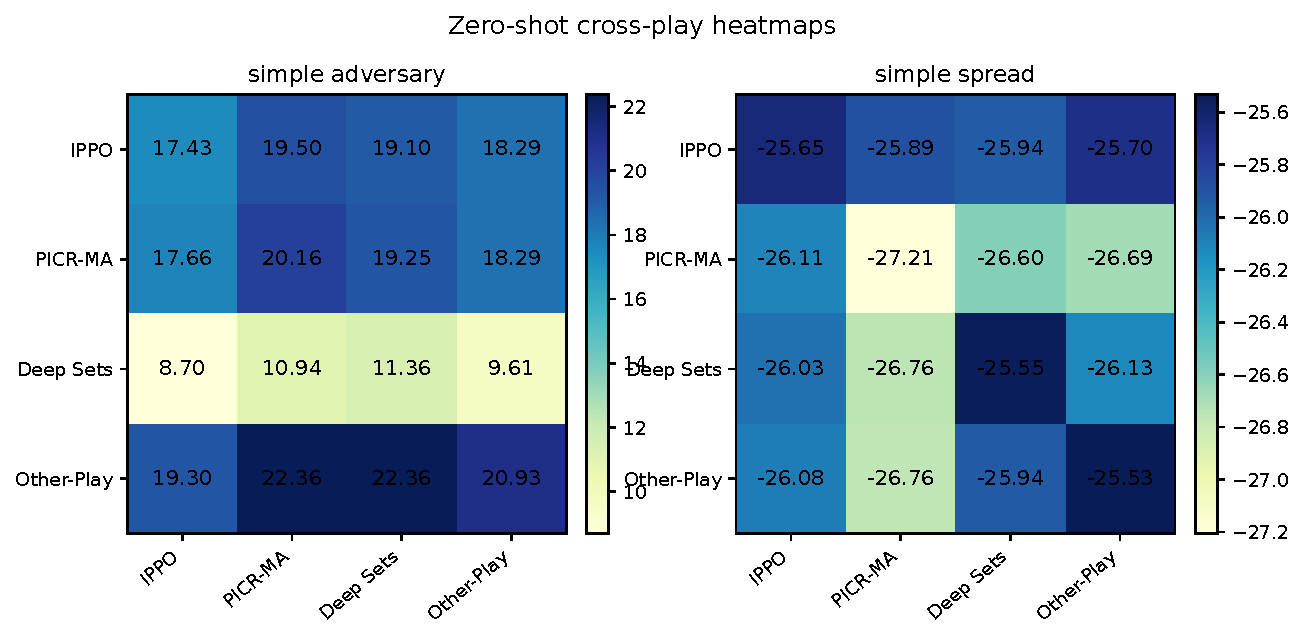
\includegraphics[width=0.92\linewidth]{latex/figures/zero_shot_crossplay_results.pdf}
\caption{Held-out partner cross-play heatmaps from the main 50k cohort. The main paper uses a compact summary plot; this appendix figure exposes the full family-by-family structure.}
\label{fig:heatmaps}
\end{figure*}

\section{Additional Tables}
\begin{table}[h]
\centering
\caption{Held-out partner cross-play split into same-family and cross-family partners.}
\begin{tabular}{llcc}
\toprule
Environment & Ego method & Same-family & Cross-family \\
\midrule
Simple Adversary & Deep Sets & 11.356 $\pm$ 2.239 & 9.751 $\pm$ 1.260 \\
Simple Adversary & IPPO & 17.429 $\pm$ 2.729 & 18.964 $\pm$ 1.501 \\
Simple Adversary & Other-Play & \textbf{20.934 $\pm$ 2.639} & \textbf{21.342 $\pm$ 1.253} \\
Simple Adversary & PICR-MA & 20.159 $\pm$ 2.398 & 18.400 $\pm$ 1.084 \\
Simple Spread & Deep Sets & -25.550 $\pm$ 0.910 & -26.305 $\pm$ 0.361 \\
Simple Spread & IPPO & -25.649 $\pm$ 0.584 & \textbf{-25.844 $\pm$ 0.438} \\
Simple Spread & Other-Play & \textbf{-25.533 $\pm$ 0.782} & -26.260 $\pm$ 0.437 \\
Simple Spread & PICR-MA & -27.206 $\pm$ 0.702 & -26.466 $\pm$ 0.454 \\
\bottomrule
\end{tabular}

\end{table}

\begin{table}[h]
\centering
\caption{Matched-seed PICR-MA versus IPPO deltas. The cross-play rows report same-family held-out partner cross-play, and negative $\Delta$JS is desirable. The table makes the workshop claim explicit: the diagnostic shift is more consistent than the coordination shift.}
\resizebox{\linewidth}{!}{\begin{tabular}{llccc}
\toprule
Environment & Quantity & Mean delta & 95\% bootstrap CI & Direction count \\
\midrule
Simple Spread & Same-family cross-play & -1.557 & [-3.013, -0.651] & 0/5 higher \\
Simple Spread & JS $\downarrow$ & -0.014 & [-0.027, -0.004] & 5/5 lower \\
\midrule
Simple Adversary & Same-family cross-play & 2.731 & [-6.141, 12.263] & 3/5 higher \\
Simple Adversary & JS $\downarrow$ & -0.005 & [-0.015, 0.002] & 4/5 lower \\
\bottomrule
\end{tabular}
}
\end{table}

\begin{table}[h]
\centering
\caption{Permutation sensitivity summary across environments and methods.}
\begin{tabular}{llc}
\toprule
Environment & Method & JS divergence \\
\midrule
Simple Adversary & Deep Sets & \textbf{0.000 $\pm$ 0.000} \\
Simple Adversary & IPPO & 0.010 $\pm$ 0.001 \\
Simple Adversary & Other-Play & 0.014 $\pm$ 0.001 \\
Simple Adversary & PICR-MA & 0.005 $\pm$ 0.001 \\
Simple Spread & Deep Sets & \textbf{0.000 $\pm$ 0.000} \\
Simple Spread & IPPO & 0.026 $\pm$ 0.001 \\
Simple Spread & Other-Play & 0.025 $\pm$ 0.003 \\
Simple Spread & PICR-MA & 0.013 $\pm$ 0.001 \\
\bottomrule
\end{tabular}

\end{table}

\begin{table}[h]
\centering
\caption{Runtime summary relative to IPPO.}
\begin{tabular}{llcc}
\toprule
Environment & Method & Runtime (s) & Relative to IPPO \\
\midrule
Simple Adversary & Deep Sets & 44.885 & 1.34$\times$ \\
Simple Adversary & IPPO & 33.504 & 1.00$\times$ \\
Simple Adversary & Other-Play & \textbf{32.045} & 0.96$\times$ \\
Simple Adversary & PICR-MA & 44.575 & 1.33$\times$ \\
Simple Spread & Deep Sets & 62.529 & 2.02$\times$ \\
Simple Spread & IPPO & \textbf{31.004} & 1.00$\times$ \\
Simple Spread & Other-Play & 32.329 & 1.04$\times$ \\
Simple Spread & PICR-MA & 50.235 & 1.62$\times$ \\
\bottomrule
\end{tabular}

\end{table}

\section{Matrix-Game Sanity Checks}
The matrix games remain useful as fast debugging environments for observation slicing, partner-pool evaluation, and rollout correctness, but they do not determine the paper's main claim. We therefore treat them as supporting evidence rather than headline evidence.

\begin{figure}[h]
\centering
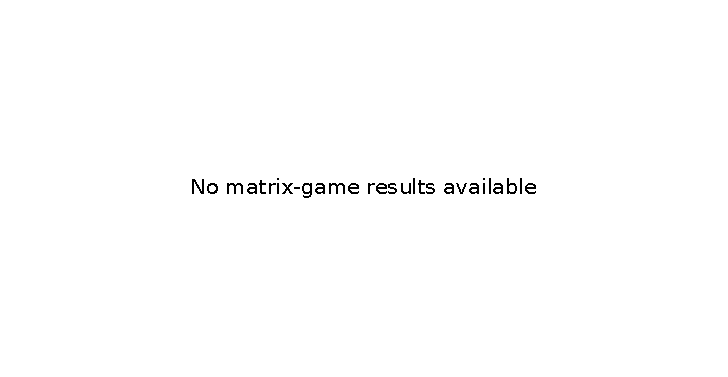
\includegraphics[width=\linewidth]{latex/figures/optional_matrix_games_summary.pdf}
\caption{Matrix-game summary under the current small-compute regime.}
\label{fig:matrix}
\end{figure}

\section{Observation Slicing, Hyperparameters, and Assets}
\paragraph{Observation slicing.}
Teammate-block indices are explicitly cached per environment rather than inferred implicitly at each update. For \texttt{simple\_adversary\_v3}, the consistency loss is applied only to the cooperative team. The precise slicing assumptions and any environment-specific simplifications are recorded in \texttt{results/OVERRIDES.md}.

\paragraph{Hyperparameters.}
The main reported learner uses hidden size 64, learning rate $3\times 10^{-3}$, discount 0.99, GAE parameter 0.95, PPO clip ratio 0.2, and four update epochs per rollout. The main PICR-MA cohort uses $\lambda=0.02$ and no teammate dropout. Exact commands, profiles, and artifact inventories are listed in \texttt{results/FINAL\_REPORT.md}.

\paragraph{Model capacity and fairness.}
IPPO, PICR-MA, and Other-Play share the same inference-time MLP and optimizer settings; only Deep Sets changes the encoder capacity. In the main cohort this corresponds to 1606 cooperative parameters for IPPO/PICR-MA/Other-Play versus 3302 for Deep Sets on \texttt{simple\_spread\_v3}, and 1350 versus 3238 on \texttt{simple\_adversary\_v3}. PICR-MA's extra runtime therefore comes from training-time consistency passes rather than a larger deployed policy.

\paragraph{Assets and licenses.}
The experiments rely on PettingZoo 1.24.3, Gymnasium 1.2.3, and SuperSuit 3.10.0. Local package metadata reports MIT licenses for these core environment assets. All reported figures and tables are generated from files stored under \texttt{results/}.

\section*{NeurIPS Paper Checklist}

\begin{enumerate}

\item {\bf Claims}
    \item[] Question: Do the main claims made in the abstract and introduction accurately reflect the paper's contributions and scope?
    \item[] Answer: \answerYes{}
    \item[] Justification: The abstract and introduction state the paper's scope narrowly and match the empirical evidence: PICR-MA lowers permutation sensitivity, helps on one MPE task, hurts on another, and does not support a universal ZSC claim.
    \item[] Guidelines:
    \begin{itemize}
        \item The answer \answerNA{} means that the abstract and introduction do not include the claims made in the paper.
        \item The abstract and/or introduction should clearly state the claims made, including the contributions made in the paper and important assumptions and limitations. A \answerNo{} or \answerNA{} answer to this question will not be perceived well by the reviewers. 
        \item The claims made should match theoretical and experimental results, and reflect how much the results can be expected to generalize to other settings. 
        \item It is fine to include aspirational goals as motivation as long as it is clear that these goals are not attained by the paper. 
    \end{itemize}

\item {\bf Limitations}
    \item[] Question: Does the paper discuss the limitations of the work performed by the authors?
    \item[] Answer: \answerYes{}
    \item[] Justification: The Discussion section explicitly covers the small-compute regime, the NumPy learner, the 50k-step scale limit, and the mixed baseline outcomes.
    \item[] Guidelines:
    \begin{itemize}
        \item The answer \answerNA{} means that the paper has no limitation while the answer \answerNo{} means that the paper has limitations, but those are not discussed in the paper. 
        \item The authors are encouraged to create a separate ``Limitations'' section in their paper.
        \item The paper should point out any strong assumptions and how robust the results are to violations of these assumptions (e.g., independence assumptions, noiseless settings, model well-specification, asymptotic approximations only holding locally). The authors should reflect on how these assumptions might be violated in practice and what the implications would be.
        \item The authors should reflect on the scope of the claims made, e.g., if the approach was only tested on a few datasets or with a few runs. In general, empirical results often depend on implicit assumptions, which should be articulated.
        \item The authors should reflect on the factors that influence the performance of the approach. For example, a facial recognition algorithm may perform poorly when image resolution is low or images are taken in low lighting. Or a speech-to-text system might not be used reliably to provide closed captions for online lectures because it fails to handle technical jargon.
        \item The authors should discuss the computational efficiency of the proposed algorithms and how they scale with dataset size.
        \item If applicable, the authors should discuss possible limitations of their approach to address problems of privacy and fairness.
        \item While the authors might fear that complete honesty about limitations might be used by reviewers as grounds for rejection, a worse outcome might be that reviewers discover limitations that aren't acknowledged in the paper. The authors should use their best judgment and recognize that individual actions in favor of transparency play an important role in developing norms that preserve the integrity of the community. Reviewers will be specifically instructed to not penalize honesty concerning limitations.
    \end{itemize}

\item {\bf Theory assumptions and proofs}
    \item[] Question: For each theoretical result, does the paper provide the full set of assumptions and a complete (and correct) proof?
    \item[] Answer: \answerNA{}
    \item[] Justification: The paper is empirical and does not present new formal theorems or proofs.
    \item[] Guidelines:
    \begin{itemize}
        \item The answer \answerNA{} means that the paper does not include theoretical results. 
        \item All the theorems, formulas, and proofs in the paper should be numbered and cross-referenced.
        \item All assumptions should be clearly stated or referenced in the statement of any theorems.
        \item The proofs can either appear in the main paper or the supplemental material, but if they appear in the supplemental material, the authors are encouraged to provide a short proof sketch to provide intuition. 
        \item Inversely, any informal proof provided in the core of the paper should be complemented by formal proofs provided in appendix or supplemental material.
        \item Theorems and Lemmas that the proof relies upon should be properly referenced. 
    \end{itemize}

    \item {\bf Experimental result reproducibility}
    \item[] Question: Does the paper fully disclose all the information needed to reproduce the main experimental results of the paper to the extent that it affects the main claims and/or conclusions of the paper (regardless of whether the code and data are provided or not)?
    \item[] Answer: \answerYes{}
    \item[] Justification: The paper specifies environments, baselines, seeds, steps, hyperparameters, partner-pool evaluation, and the artifact paths used to generate the figures and tables.
    \item[] Guidelines:
    \begin{itemize}
        \item The answer \answerNA{} means that the paper does not include experiments.
        \item If the paper includes experiments, a \answerNo{} answer to this question will not be perceived well by the reviewers: Making the paper reproducible is important, regardless of whether the code and data are provided or not.
        \item If the contribution is a dataset and\slash or model, the authors should describe the steps taken to make their results reproducible or verifiable. 
        \item Depending on the contribution, reproducibility can be accomplished in various ways. For example, if the contribution is a novel architecture, describing the architecture fully might suffice, or if the contribution is a specific model and empirical evaluation, it may be necessary to either make it possible for others to replicate the model with the same dataset, or provide access to the model. In general. releasing code and data is often one good way to accomplish this, but reproducibility can also be provided via detailed instructions for how to replicate the results, access to a hosted model (e.g., in the case of a large language model), releasing of a model checkpoint, or other means that are appropriate to the research performed.
        \item While NeurIPS does not require releasing code, the conference does require all submissions to provide some reasonable avenue for reproducibility, which may depend on the nature of the contribution. For example
        \begin{enumerate}
            \item If the contribution is primarily a new algorithm, the paper should make it clear how to reproduce that algorithm.
            \item If the contribution is primarily a new model architecture, the paper should describe the architecture clearly and fully.
            \item If the contribution is a new model (e.g., a large language model), then there should either be a way to access this model for reproducing the results or a way to reproduce the model (e.g., with an open-source dataset or instructions for how to construct the dataset).
            \item We recognize that reproducibility may be tricky in some cases, in which case authors are welcome to describe the particular way they provide for reproducibility. In the case of closed-source models, it may be that access to the model is limited in some way (e.g., to registered users), but it should be possible for other researchers to have some path to reproducing or verifying the results.
        \end{enumerate}
    \end{itemize}


\item {\bf Open access to data and code}
    \item[] Question: Does the paper provide open access to the data and code, with sufficient instructions to faithfully reproduce the main experimental results, as described in supplemental material?
    \item[] Answer: \answerYes{}
    \item[] Justification: The submission package includes the code, generated results, and scripts used for training, evaluation, aggregation, plots, tables, and manuscript population, together with report files documenting exact commands.
    \item[] Guidelines:
    \begin{itemize}
        \item The answer \answerNA{} means that paper does not include experiments requiring code.
        \item Please see the NeurIPS code and data submission guidelines (\url{https://neurips.cc/public/guides/CodeSubmissionPolicy}) for more details.
        \item While we encourage the release of code and data, we understand that this might not be possible, so \answerNo{} is an acceptable answer. Papers cannot be rejected simply for not including code, unless this is central to the contribution (e.g., for a new open-source benchmark).
        \item The instructions should contain the exact command and environment needed to run to reproduce the results. See the NeurIPS code and data submission guidelines (\url{https://neurips.cc/public/guides/CodeSubmissionPolicy}) for more details.
        \item The authors should provide instructions on data access and preparation, including how to access the raw data, preprocessed data, intermediate data, and generated data, etc.
        \item The authors should provide scripts to reproduce all experimental results for the new proposed method and baselines. If only a subset of experiments are reproducible, they should state which ones are omitted from the script and why.
        \item At submission time, to preserve anonymity, the authors should release anonymized versions (if applicable).
        \item Providing as much information as possible in supplemental material (appended to the paper) is recommended, but including URLs to data and code is permitted.
    \end{itemize}


\item {\bf Experimental setting/details}
    \item[] Question: Does the paper specify all the training and test details (e.g., data splits, hyperparameters, how they were chosen, type of optimizer) necessary to understand the results?
    \item[] Answer: \answerYes{}
    \item[] Justification: The main text reports the learner family, environment setup, evaluation protocol, and hyperparameter-selection logic, and the appendix points to exact config files and run reports.
    \item[] Guidelines:
    \begin{itemize}
        \item The answer \answerNA{} means that the paper does not include experiments.
        \item The experimental setting should be presented in the core of the paper to a level of detail that is necessary to appreciate the results and make sense of them.
        \item The full details can be provided either with the code, in appendix, or as supplemental material.
    \end{itemize}

\item {\bf Experiment statistical significance}
    \item[] Question: Does the paper report error bars suitably and correctly defined or other appropriate information about the statistical significance of the experiments?
    \item[] Answer: \answerYes{}
    \item[] Justification: The main-paper figures and tables report mean $\pm$ standard error across seeds or partner samples, and the paper states that the uncertainties are standard errors rather than significance tests.
    \item[] Guidelines:
    \begin{itemize}
        \item The answer \answerNA{} means that the paper does not include experiments.
        \item The authors should answer \answerYes{} if the results are accompanied by error bars, confidence intervals, or statistical significance tests, at least for the experiments that support the main claims of the paper.
        \item The factors of variability that the error bars are capturing should be clearly stated (for example, train/test split, initialization, random drawing of some parameter, or overall run with given experimental conditions).
        \item The method for calculating the error bars should be explained (closed form formula, call to a library function, bootstrap, etc.)
        \item The assumptions made should be given (e.g., Normally distributed errors).
        \item It should be clear whether the error bar is the standard deviation or the standard error of the mean.
        \item It is OK to report 1-sigma error bars, but one should state it. The authors should preferably report a 2-sigma error bar than state that they have a 96\% CI, if the hypothesis of Normality of errors is not verified.
        \item For asymmetric distributions, the authors should be careful not to show in tables or figures symmetric error bars that would yield results that are out of range (e.g., negative error rates).
        \item If error bars are reported in tables or plots, the authors should explain in the text how they were calculated and reference the corresponding figures or tables in the text.
    \end{itemize}

\item {\bf Experiments compute resources}
    \item[] Question: For each experiment, does the paper provide sufficient information on the computer resources (type of compute workers, memory, time of execution) needed to reproduce the experiments?
    \item[] Answer: \answerYes{}
    \item[] Justification: The paper reports the Apple Silicon laptop setting, the lean-safe resource profile, and per-run wall-clock runtime, and it notes that all experiments were executed sequentially on local compute.
    \item[] Guidelines:
    \begin{itemize}
        \item The answer \answerNA{} means that the paper does not include experiments.
        \item The paper should indicate the type of compute workers CPU or GPU, internal cluster, or cloud provider, including relevant memory and storage.
        \item The paper should provide the amount of compute required for each of the individual experimental runs as well as estimate the total compute. 
        \item The paper should disclose whether the full research project required more compute than the experiments reported in the paper (e.g., preliminary or failed experiments that didn't make it into the paper). 
    \end{itemize}
    
\item {\bf Code of ethics}
    \item[] Question: Does the research conducted in the paper conform, in every respect, with the NeurIPS Code of Ethics \url{https://neurips.cc/public/EthicsGuidelines}?
    \item[] Answer: \answerYes{}
    \item[] Justification: The work is a small-scale empirical study on open-source simulated environments and does not involve deception, human subjects, or restricted data.
    \item[] Guidelines:
    \begin{itemize}
        \item The answer \answerNA{} means that the authors have not reviewed the NeurIPS Code of Ethics.
        \item If the authors answer \answerNo, they should explain the special circumstances that require a deviation from the Code of Ethics.
        \item The authors should make sure to preserve anonymity (e.g., if there is a special consideration due to laws or regulations in their jurisdiction).
    \end{itemize}


\item {\bf Broader impacts}
    \item[] Question: Does the paper discuss both potential positive societal impacts and negative societal impacts of the work performed?
    \item[] Answer: \answerYes{}
    \item[] Justification: The paper includes a broader-impact discussion covering both improved robustness/reproducibility and possible risks from broader deployment of multi-agent systems.
    \item[] Guidelines:
    \begin{itemize}
        \item The answer \answerNA{} means that there is no societal impact of the work performed.
        \item If the authors answer \answerNA{} or \answerNo, they should explain why their work has no societal impact or why the paper does not address societal impact.
        \item Examples of negative societal impacts include potential malicious or unintended uses (e.g., disinformation, generating fake profiles, surveillance), fairness considerations (e.g., deployment of technologies that could make decisions that unfairly impact specific groups), privacy considerations, and security considerations.
        \item The conference expects that many papers will be foundational research and not tied to particular applications, let alone deployments. However, if there is a direct path to any negative applications, the authors should point it out. For example, it is legitimate to point out that an improvement in the quality of generative models could be used to generate Deepfakes for disinformation. On the other hand, it is not needed to point out that a generic algorithm for optimizing neural networks could enable people to train models that generate Deepfakes faster.
        \item The authors should consider possible harms that could arise when the technology is being used as intended and functioning correctly, harms that could arise when the technology is being used as intended but gives incorrect results, and harms following from (intentional or unintentional) misuse of the technology.
        \item If there are negative societal impacts, the authors could also discuss possible mitigation strategies (e.g., gated release of models, providing defenses in addition to attacks, mechanisms for monitoring misuse, mechanisms to monitor how a system learns from feedback over time, improving the efficiency and accessibility of ML).
    \end{itemize}
    
\item {\bf Safeguards}
    \item[] Question: Does the paper describe safeguards that have been put in place for responsible release of data or models that have a high risk for misuse (e.g., pre-trained language models, image generators, or scraped datasets)?
    \item[] Answer: \answerNA{}
    \item[] Justification: The paper does not release high-risk generative models, scraped datasets, or similarly dual-use assets.
    \item[] Guidelines:
    \begin{itemize}
        \item The answer \answerNA{} means that the paper poses no such risks.
        \item Released models that have a high risk for misuse or dual-use should be released with necessary safeguards to allow for controlled use of the model, for example by requiring that users adhere to usage guidelines or restrictions to access the model or implementing safety filters. 
        \item Datasets that have been scraped from the Internet could pose safety risks. The authors should describe how they avoided releasing unsafe images.
        \item We recognize that providing effective safeguards is challenging, and many papers do not require this, but we encourage authors to take this into account and make a best faith effort.
    \end{itemize}

\item {\bf Licenses for existing assets}
    \item[] Question: Are the creators or original owners of assets (e.g., code, data, models), used in the paper, properly credited and are the license and terms of use explicitly mentioned and properly respected?
    \item[] Answer: \answerYes{}
    \item[] Justification: The paper cites the environment and baseline sources and the appendix records the locally verified MIT license metadata for the core environment packages used in the study.
    \item[] Guidelines:
    \begin{itemize}
        \item The answer \answerNA{} means that the paper does not use existing assets.
        \item The authors should cite the original paper that produced the code package or dataset.
        \item The authors should state which version of the asset is used and, if possible, include a URL.
        \item The name of the license (e.g., CC-BY 4.0) should be included for each asset.
        \item For scraped data from a particular source (e.g., website), the copyright and terms of service of that source should be provided.
        \item If assets are released, the license, copyright information, and terms of use in the package should be provided. For popular datasets, \url{paperswithcode.com/datasets} has curated licenses for some datasets. Their licensing guide can help determine the license of a dataset.
        \item For existing datasets that are re-packaged, both the original license and the license of the derived asset (if it has changed) should be provided.
        \item If this information is not available online, the authors are encouraged to reach out to the asset's creators.
    \end{itemize}

\item {\bf New assets}
    \item[] Question: Are new assets introduced in the paper well documented and is the documentation provided alongside the assets?
    \item[] Answer: \answerYes{}
    \item[] Justification: The repository documents the new code, result artifacts, and manuscript exports with a README, run reports, and explicit reproduction commands.
    \item[] Guidelines:
    \begin{itemize}
        \item The answer \answerNA{} means that the paper does not release new assets.
        \item Researchers should communicate the details of the dataset\slash code\slash model as part of their submissions via structured templates. This includes details about training, license, limitations, etc. 
        \item The paper should discuss whether and how consent was obtained from people whose asset is used.
        \item At submission time, remember to anonymize your assets (if applicable). You can either create an anonymized URL or include an anonymized zip file.
    \end{itemize}

\item {\bf Crowdsourcing and research with human subjects}
    \item[] Question: For crowdsourcing experiments and research with human subjects, does the paper include the full text of instructions given to participants and screenshots, if applicable, as well as details about compensation (if any)? 
    \item[] Answer: \answerNA{}
    \item[] Justification: The work does not involve crowdsourcing or human-subject data collection.
    \item[] Guidelines:
    \begin{itemize}
        \item The answer \answerNA{} means that the paper does not involve crowdsourcing nor research with human subjects.
        \item Including this information in the supplemental material is fine, but if the main contribution of the paper involves human subjects, then as much detail as possible should be included in the main paper. 
        \item According to the NeurIPS Code of Ethics, workers involved in data collection, curation, or other labor should be paid at least the minimum wage in the country of the data collector. 
    \end{itemize}

\item {\bf Institutional review board (IRB) approvals or equivalent for research with human subjects}
    \item[] Question: Does the paper describe potential risks incurred by study participants, whether such risks were disclosed to the subjects, and whether Institutional Review Board (IRB) approvals (or an equivalent approval/review based on the requirements of your country or institution) were obtained?
    \item[] Answer: \answerNA{}
    \item[] Justification: The reported experiments are entirely in simulation and do not involve human participants.
    \item[] Guidelines:
    \begin{itemize}
        \item The answer \answerNA{} means that the paper does not involve crowdsourcing nor research with human subjects.
        \item Depending on the country in which research is conducted, IRB approval (or equivalent) may be required for any human subjects research. If you obtained IRB approval, you should clearly state this in the paper. 
        \item We recognize that the procedures for this may vary significantly between institutions and locations, and we expect authors to adhere to the NeurIPS Code of Ethics and the guidelines for their institution. 
        \item For initial submissions, do not include any information that would break anonymity (if applicable), such as the institution conducting the review.
    \end{itemize}

\item {\bf Declaration of LLM usage}
    \item[] Question: Does the paper describe the usage of LLMs if it is an important, original, or non-standard component of the core methods in this research? Note that if the LLM is used only for writing, editing, or formatting purposes and does \emph{not} impact the core methodology, scientific rigor, or originality of the research, declaration is not required.
    %this research? 
    \item[] Answer: \answerNA{}
    \item[] Justification: LLMs are not part of the method, training pipeline, or experimental claims in this paper.
    \item[] Guidelines:
    \begin{itemize}
        \item The answer \answerNA{} means that the core method development in this research does not involve LLMs as any important, original, or non-standard components.
        \item Please refer to our LLM policy in the NeurIPS handbook for what should or should not be described.
    \end{itemize}

\end{enumerate}


\end{document}
